%%
% Please see https://bitbucket.org/rivanvx/beamer/wiki/Home for obtaining beamer.
%%
\documentclass{beamer}

\usepackage{braket}
\usepackage{graphicx}
% \usepackage{tikz}
\usepackage{pgfplots}
\usepackage{adjustbox}
\usepackage{xcolor}

\definecolor{grn}{RGB}{34,139,34}

\pgfplotsset{width=10cm,compat=1.9}


\DeclareMathOperator{\val}{val}
\DeclareMathOperator{\trop}{trop}
\DeclareMathOperator{\initial}{in}

\newcommand{\R}{\ensuremath{\mathbb{R}}}
\newcommand{\Q}{\ensuremath{\mathbb{Q}}}
\newcommand{\N}{\ensuremath{\mathbb{N}}}
\newcommand{\C}{\ensuremath{\mathbb{C}}}
\newcommand{\PS}{\ensuremath{ \C \{\{ t \} \} }}


\usetheme{Madrid}

\title{Elements of Tropical Geometry}
\author{Jack Maloney}

\begin{document}

\begin{frame}
\titlepage
\end{frame}

\begin{frame}{Why Tropical?}
	\begin{figure}
		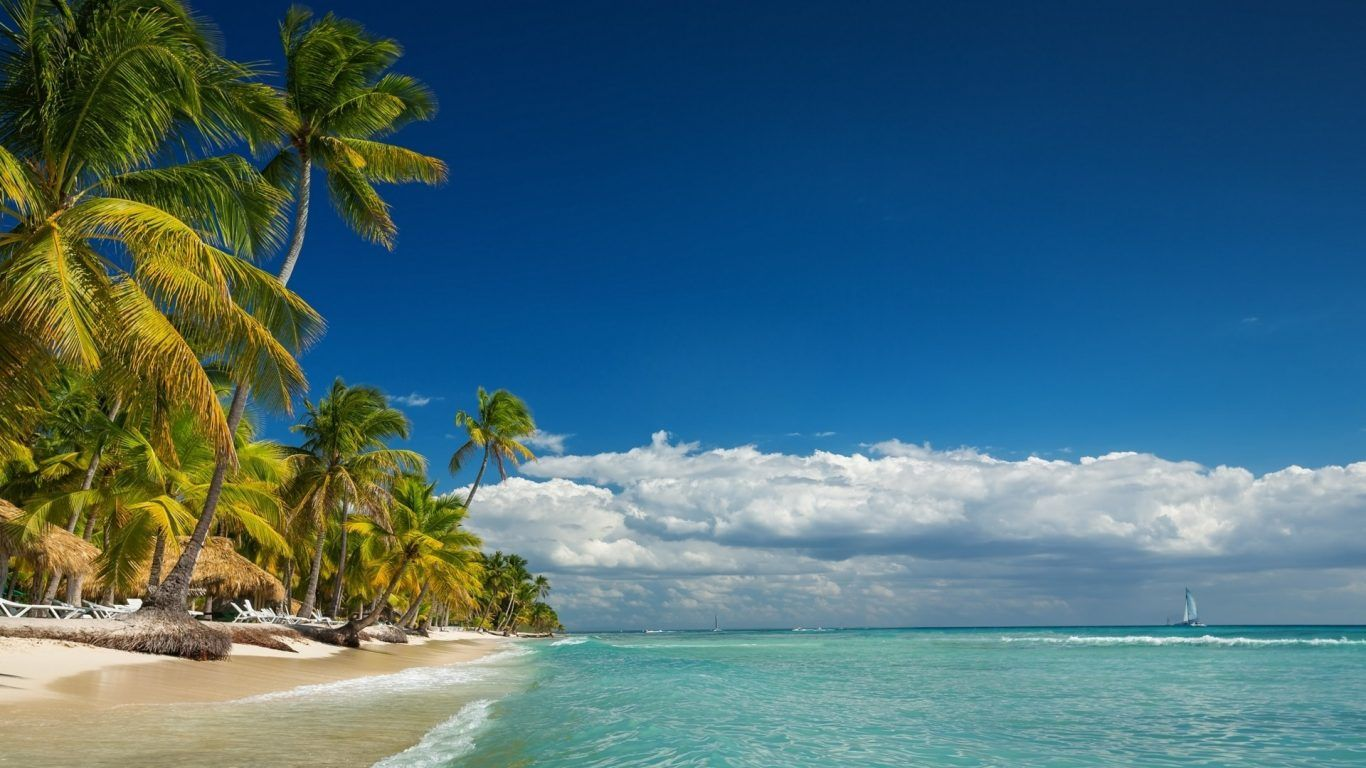
\includegraphics[width=\textwidth]{tropical.jpg}
	\end{figure}
\end{frame}

\begin{frame}{Tropical Geometry}
	\begin{enumerate}
	    \item Classical Algebraic Geometry
	    \begin{align}
	        V(f_1, ..., f_k) = \Set { (x_0, ..., x_n) \in \R^n | f_i(x) = 0 \text{ for all } i }
	    \end{align}
	    % Fields other than R ok.
	    \pause
		\item Simplify Algebraic Geometry
			\begin{align}
				\text{complicated classical variety} \rightarrow \text{simplified tropical variety}
			\end{align}
		\pause
		Hopefully retains some geometric information about the classical variety we are interested in.
		\pause
		\item Tropical Semiring
		\begin{align}
			\left( \R \cup \Set{ + \infty }, \oplus, \odot \right) 
		\end{align}
		\pause
		\vspace{-2.5em}
		\begin{align}
			x \oplus y = \min \Set{x, y}
			\quad \text{and} \quad 
			x \odot y = x + y
		\end{align}
		%  Tropical Exponentiation? 
	\end{enumerate}
\end{frame}

% \begin{frame}{Field with Valuation}
%     %% Laurent Series, no field, just valuation.

% 	A \textbf{Valuation} on a field \( K \) is a map \( \val : K \rightarrow \R \cup \Set{ + \infty } \) which satisfies the following axioms
% 	\begin{enumerate}
% 		\item \( \val (a) = \infty \) iff \( a = 0 \)
% 		\item \( \val ( a b ) = \val (a) + \val (b) \)
% 		\item \( \val ( a + b ) \geq \min \Set { \val(a), \val(b) } \)
% 	\end{enumerate}

% 	\pause
% 	\begin{block}{\textbf{Example:} Trivial valuation}
% 	    Let \( val(a) = 0\) for all \( a \in K^* \).
% 	\end{block}
	
% 	\pause
% 	Valuations help retain some geometric information when converting to tropical varieties.
	
% %	\pause
% %	\begin{block}{\textbf{Example:} \( \Q \) with p-adic valuation}
% %	Fix a prime number \(p\). Then define 
% %	\end{block}

% \end{frame}

\begin{frame}{Tropicalization of a Polynomial}
    % Simplify this!
    % Classical operations -> Tropical Operations.
    % Go straight to example
% 	\begin{align}
% 		f(x) = \sum_{\textbf{u} \in \N ^{n}} 
% 			a_{\textbf{u}} x^{\textbf{u}}
% 		\in K[x_0, ..., x_{n-1}]
% 	\end{align}

% 	\pause
% 	Then
% 	\begin{align}
% 		\trop(f)(x) 
% 		& = \bigoplus_{\textbf{u} \in \N^{n}} 
% 			\val(a_{\textbf{u}}) \odot \left( x \cdot \textbf{u} \right) \\
% 		& = \min_{\textbf{u} \in \N ^{n}} \Set{ \val(a_{\textbf{u}}) + \left( x \cdot \textbf{u} \right) }
% 		\in \R[x_0, ..., x_{n-1}]
% 	\end{align}

    Replace classical arithmetic operations with tropical versions.
    \begin{enumerate}
        \item Coefficents get mapped to the tropical semiring via a \textit{valuation}
        \item Addition becomes minimization
        \item Multiplication becomes addition
        \item Exponentiation becomes multiplication/dot product
    \end{enumerate}

	\pause
	\begin{align}
	    \text{classical polynomial on } K^n \quad \rightarrow \quad \text{piecewise linear function on } \R^n
	\end{align}
	
	\pause
	\begin{align}
		\text{monomials are products} \quad \rightarrow \quad \text{monomials are sums (tropical products)}
	\end{align}
\end{frame}

\begin{frame}{Example}
    % Color corresponding exponents/valuations/variables/etc
    \begin{align}
        f(x) = 
        ({\textcolor{magenta}{t}}) x^{\textcolor{grn}{2}} +
        ({\textcolor{magenta}{t^{-2} + t}}) x^{\textcolor{grn}{1}} +
        ({\textcolor{magenta}{t^2}}) x^{\textcolor{grn}{0}} 
        \in \PS [x]
    \end{align}

    \pause
    \begin{align}
        \trop(f)(x)
        = \min \Set{ 
            \val({\textcolor{magenta}{t}}) + {\textcolor{grn}{2}}x, 
            \, \val({\textcolor{magenta}{t^{-2} + t}}) + {\textcolor{grn}{1}} x, 
            \, \val({\textcolor{magenta}{t^2}}) + {\textcolor{grn}{0}} x }
    \end{align}

    \pause
    \begin{align}
        = \min \Set{ 
            {\textcolor{magenta}{1}} + {\textcolor{grn}{2}}x, 
            \, {\textcolor{magenta}{-2}} + {\textcolor{grn}{1}}x, 
            \, {\textcolor{magenta}{2}} + {\textcolor{grn}{0}}x }
    \end{align}
\end{frame}

\begin{frame}{Example}
\begin{align}
    \trop(f)(x) = \min \Set{ 
                1 + 2x, \,
                x - 2, \, 
                2 }
\end{align}
% Highlight the non-differentiable points here? Talk about them being important. Multiple tropical monomials reaching the minimum simultaneously
\begin{adjustbox}{max totalsize={\textwidth}{.7\textheight},center}
    \centering
    \begin{tikzpicture}
        \begin{axis}[
                axis lines = center,
                xlabel = \(x\),
                ylabel = {\(f(x)\)},
            ]
    
            \addplot [
                domain=-7:7,
                samples=100, 
                color=blue,
                line width=0.5mm
                ]
                {min( 1 + 2 * x, x - 2, 2 )};
            % \addlegendentry{\(\trop(f)(x) = \min \Set{ 0 + 2x, 0 + x, 0 + 0 }\)}
            \draw [red, ->, line width=1mm] (axis cs: -4, -3.5) -- (axis cs: -3.1, -4.8);
            \draw [red, ->, line width=1mm] (axis cs: 5, 0.5) -- (axis cs: 4.1, 1.9);

        \end{axis}
    \end{tikzpicture}
\end{adjustbox}
\end{frame}

\begin{frame}{Tropical Varieties}
	We call the set of points where the minimum in the tropicalization is reached twice or more the \ \textbf{Tropical Variety} of \(f\), written \( \trop (V(f)) \).
	
	\vspace{4em}
	\pause
	In the example before,
	\begin{align}
	    \trop (V(f)) = \Set { -3 , 4 }
	\end{align}
	
	\pause
	These are exactly the non-differentiable points of the tropicalization.
	
\end{frame}

% \begin{frame}{Initial Forms}
%     Given a polynomial
% 	\begin{align}
% 		f(x) = \sum_{\textbf{u} \in \N ^{n}} 
% 			a_{\textbf{u}} x^{\textbf{u}}
% 		\in K[x_0, ..., x_{n-1}]
% 	\end{align}
% 	\pause
% 	The \textbf{Initial Form at \(w \in \R^n \)} of a polynomial \(f\) is the term in the tropicalization of \(f\) which achieve the minimum. If there are more than one term that simultaneously achieve the minimum at \(w\), the initial form at \(w\) is their sum.
% 	\pause
% 	\begin{align}
% 	    \trop(f)(x) & = \min \Set{ 1 + 2x, \, x - 2, \, 2 }
% 	\end{align}
% 	\begin{align}
% 	    \initial_{1}(f) & = x - 2, \\
% 	    \initial_{4}(f) & = (2) + (x - 2)
% 	\end{align}
	
% 	\pause
% 	\begin{block}{Remark}
% 	    The places where the initial form has multiple terms are precisely the places where the tropicalization is not differentiable.
% 	\end{block}

% 	% Intuition of the term that meets the minimum, vs complicated formula.
	
% 	% Relate the points with multiple minimums to non-differentiable points
% 	% Grobner complexes are formed by these sections of linear minimums. Piuseaux series example would be helpful if it can be a two dimensional thing
%     % Need good example to show tropicalization and grobner complex in one go? 
% 	% Maybe get to Theorem 3.2.3 (Fundamental Theorem of Tropical Algebraic Geometry). ?
	
% \end{frame}

\begin{frame}{Example}
    % Turns out this is interesting and does relate to the original variety, even if its not immediately apparent how.
    % Also add classical vanishing?
    % Make this example a non-linear polynomial
    \begin{align}
        f(x,y) & = x^2 + y - 1 \\
        % V(f) & = \Set{ (x,y) \in \R^2 | x^2 + y - 1 = 0 } \\
        \trop(f)(x,y) & = \min \Set{ 2x, y, 0 } \\
        \trop(V(f)) & = \Set{ 2x = y \leq 0 } \cup \Set{ 2x = 0 \leq y } \cup \Set{ y = 0 \leq 2x }
    \end{align}
    \begin{adjustbox}{max totalsize={\textwidth}{.66\textheight},center}
        \begin{tikzpicture}
            \draw (0,0) -- (0,2.4);
            \draw (0,0) -- (2.4,0);
            \draw (0,0) -- (-.9, -1.8);
            
            \node[left] at (0,0) {(0,0)};
            
            \node at (1,1) {0};
            \node at (1,-1) {y};
            \node at (-1,1) {2x};
        \end{tikzpicture}
    \end{adjustbox}
    % Call this a tropical line
\end{frame}

%% Theorem 2.5.3

%% Maybe steal a result from the book relating Grobner complexes to something more tangible.

%%. Chapter 3.1 has some good figures of grobner complexes

\end{document}
